%%%%%%%%%%%%%%%%%%%%%%%%%%%%%%%% 
\section{The Field Cage and High Voltage System} 
\label{sec:detectors-fd-alt-hv}

This section describes the design of the high voltage system, field
cage and cathode for the TPC.  It is inspired from the LBNO 20-kt and
50-kt detector design, described in \anxlbnoa\ and \anxlbnob, which can
be simplified and down-sized for the DUNE detector (12~kt or 15~kt),
due to the shorter drift path and the rectangular aspect ratio of the
detector. The much shorter transversal dimension of DUNE with respect
to the LBNO design permits a lighter cathode structure (less sag
requires less compensation) and a simpler hanging system for the drift
cage and the cathode.

In the LBNO design the field cage is composed of equally spaced
octagonal rings that create a uniform drift field which have an
intensity adjustable in a range going from 500 to 1000~V/cm. This
leads, when operating at the maximal field intensity of 1~kV/cm over a
drift distance of 20~m, to a cathode voltage of up to 2~MV.

Two different approaches have been developed for the drift-field HV
system. The first approach uses an external HV power supply and uses
HV feedthroughs to penetrate into the detector volume. The WA105
demonstrator will use this approach for its drift of 6~m and a cathode
voltage up to 600~kV.  The second approach is based on a HV generator
directly inside the LAr volume, which is the the Greinacher HV
multiplier. It is an innovative technique, with some advantages
relative to the first approach. This technique particularly suits
giant-scale detectors that require a very high voltage of
$\sim$1--2~MV.

The DUNE detector (12-m drift) requires a voltage of 600~kV in order
to operate at a field intensity of 0.5~kV/cm. This voltage is a factor
of 3.3 higher than that for the reference design
(Chapter~\ref{ch:detectors-fd-ref}) and it will be tested during the
WA105 detector operation at 1~kV/cm over a 6-m drift.

The field cage designed for the LBNO 20-kt detector (20-m drift path)
is composed of 99 octagonal field-shaping coils manufactured from 316L
stainless-steel tubing and long radius elbows to EN 10217-7 shop. The
straight pipes and the elbows are assembled together to form the coils
by using a combination of welded and clamped joints.

The coils are supported by 32 off-hanging columns of G-10CR glass
fibre/epoxy-laminated sheet insulating material, built in the form of
chains and suspended from the tank deck structure.

Each coil is designed as a series of fully welded infill tubes
intended to fit between pairs of hanging support columns to form one
section of the field cage.  Short sections of the field-shaping coils
are integrated as pins into links to assemble each chain.  Longer
sections and corner sections of the field-shaping coil are then fixed
between the hanging columns to complete each coil
(Figure~\ref{fig:LBNO_FC}). The combined assembly of 99 sets of field
shaping coils within the 32 off-hanging columns provides a complete
field cage.
\begin{cdrfigure}[Assembly concept of the field cage]{LBNO_FC}
{\small Left: assembly of the elements of a hanging chain. Right: 
construction of a field cage section from the hanging chains and the field shaping coil elements.}
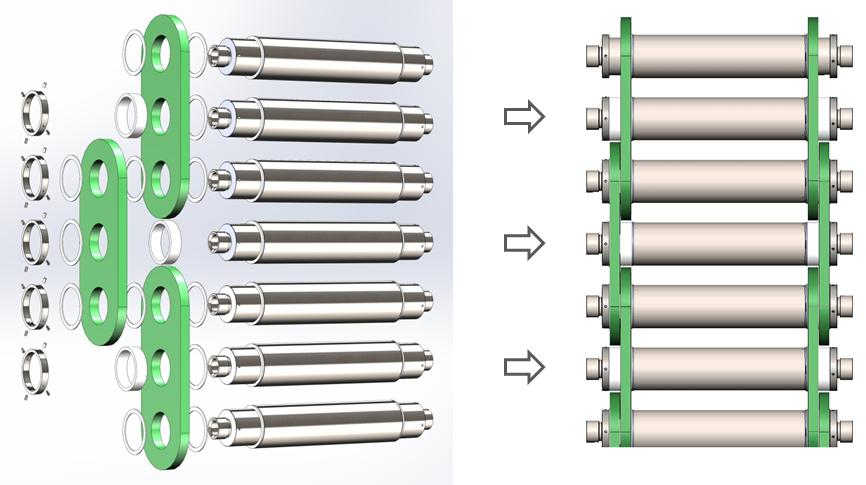
\includegraphics[width=.5\linewidth]{LBNO_chains} \hfill
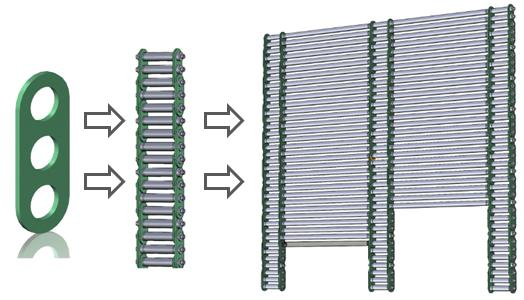
\includegraphics[width=.4\linewidth]{LBNO_FC2}
\end{cdrfigure}

The infill tube specifications assume an outer diameter of 139.7~mm,
which is common to the cathode structure.  This allows a thinner wall,
1.6~mm, to be used in non-structural parts of the coils.  Although a
non-standard size, the total length of this tube can be manufactured
as a special mill run.  This will make it possible to save 21~tons of
material relative to the standard tubes (wall thickness of
2.0~mm). The wall thickness of the link pins is 2.6~mm; this will
provide sufficient stiffness to resist to the bending torques across
the link pins.  All specialist preparation and welding of the link
pins will be carried out in shop facilities under controlled
fabrication.  This includes the rough machining of the end fittings,
preparation of the tube ends and the jig-welding of the complete
assemblies. Further machining, after welding, will be carried out to
ensure correct alignment and tolerance levels in conjunction with the
hanging columns.  Vent holes will be incorporated into the tubes as
required to facilitate construction and to allow purging with GAr/LAr
on commissioning.

Manufacturing, transportation and underground construction
considerations were a fundamental part of the field-shaping coil
design process, in collaboration with the LAGUNA-LBNO industrial
partners. The requirement of construction in a clean-room environment
within the completed membrane tank presented considerable challenges
in terms of logistics and the development of the overall concept for
fabrication.  It was concluded that a modular construction approach
would be required in order to (1) maximize off-site shop fabrication
and minimize on-site assembly, and (2) ensure the cleanliness of
construction and to minimize the installation time. The breakdown of
each field-shaping coil is made into sets of three main modules.
Although separate modules, the field shaping coils and the cathode
structure share identical features and dimensions.  Thus, the
maintenance of common interfaces is an important advantage of the
overall field cage design.
 
The DUNE 12-kt detector field cage would include 60 rectangular rings
used to cover the 12~m of drift volume.

The LBNO cathode design for the 50-kt detector follows an extensive
review of options and analysis. The design incorporates features to
minimize the static deflection of the cathode and to maximize the
electrostatic performance. (To avoid regions with high electric
fields, the electric field is limited to 50~kV/cm.)  Similar to the
field-shaping coil, and for the same reasons, the cathode is designed
as a modular structure fulfilling ensuring a minimal on-site assembly
time. The cathode is designed as a fully welded tubular rectangular
grid structure in 2~m$\times$2~m bays, 1~m deep in the vertical
direction supported only from the periphery
(Figure~\ref{fig:LBNO_cathode}).
\begin{cdrfigure}[Cathode design]{LBNO_cathode}
{\small Left: cathode plane design for the LBNO detector. Right: breakdown of 
the cathode structure in construction modules.}
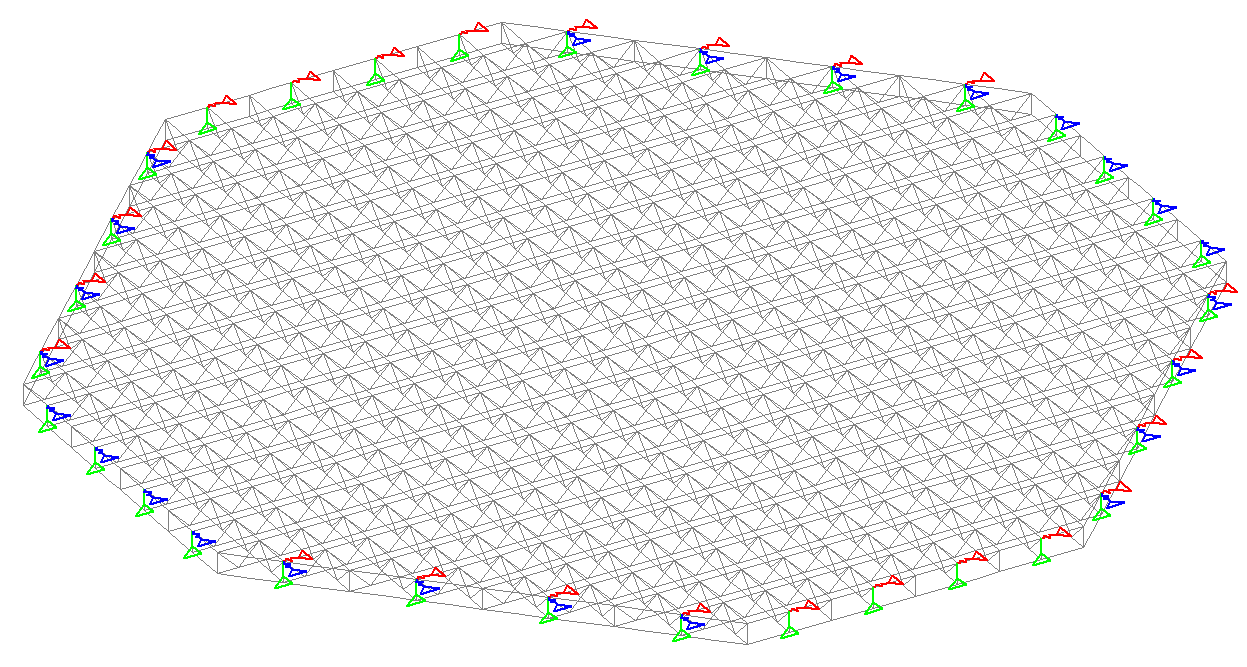
\includegraphics[width=.4\linewidth]{LBNO_cathode} \hfil
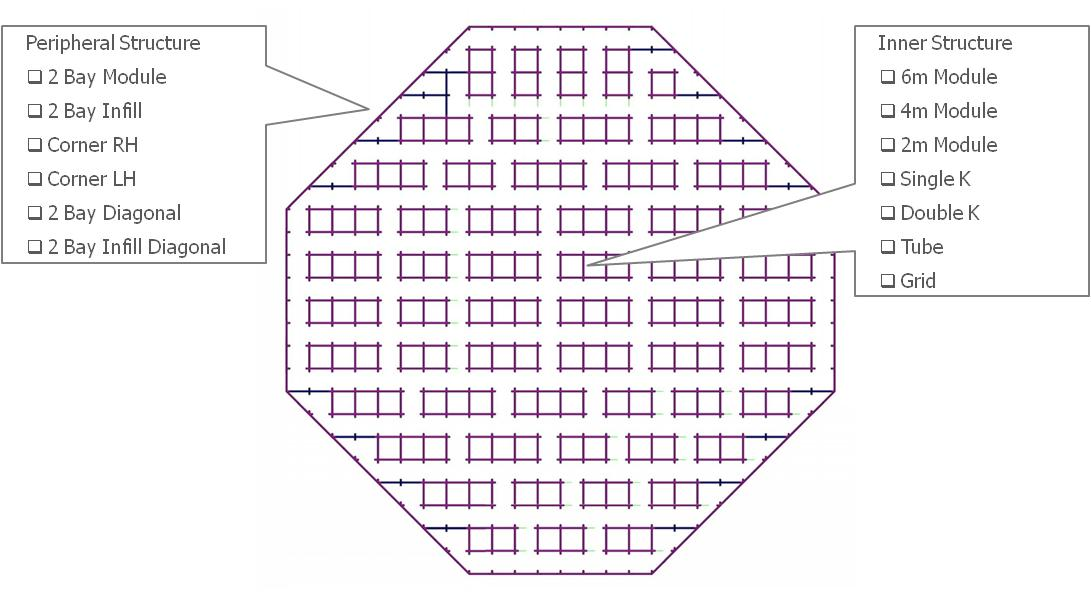
\includegraphics[width=.5\linewidth]{LBNO_cathode_elements}
\end{cdrfigure}

The top and bottom grid structures are manufactured from 139.7-mm OD
tubes with wall thickness 2.6~mm to EN 10217-7 in 316 stainless steel.
The bracing structure is manufactured from 60.3-mm OD tubes with wall
thickness 2.6~mm, also to EN 10217-7 in 316 stainless steel.  A grid
structure comprising 10-mm OD tubes with wall thickness 1~mm, arranged
in a single plane at 100-mm centers, will be fitted to the top of the
cathode only. The maximum module size for this structure is 6~m,
comprising three full 2~m$\times$2~m$\times$1~m deep bays of the
cathode structure.  All specialist nodes preparation and welding of
the modules will be carried out in controlled facilities at the
fabrication shop.  Vent holes are incorporated into the structures to
facilitate construction and to allow purging with GAr/LAr on
commissioning. High levels of quality control will be possible with
the modular construction design, and following inspection, each module
will be cleaned to ISO 8 cleanliness standard and double-wrapped prior
to dispatch and transportation to the site for installation and final
assembly.

The cathode outer top tubular structure is identical to the bottom
field-shaping coil; they use tubes of the same outer diameter
(139.7~mm).  The spans are the same (48~m for the 50-kt LBNO detector)
and the vertical distance separating these components is the same as
for the remaining field-shaping coils (200-mm centers). The cathode
will be attached at the bottom of each hanging column by a split link
in G-10CR. The cathode attachment points will also incorporate locally
thickened sections of tube (as in the hanging chains) included as part
of the peripheral structure nodes.
 
The complete assembly procedure, logistics and tooling for the field
cage and cathode is described in \anxlbnob.  It is expected that the
general design, adapted to the rectangular geometry, and the basic
elements for the cathode construction would be similar for the 12-kt
DUNE detector.  However the basic elements for the cathode
construction could be down-sized since sagging effects are only on
12~m span and not 40~m, as in the case of LBNO. This less stringent
requirement translates in a lighter and cheaper structure.
